\begin{figure*}[!t]
\centering
\definecolor{f4Blue}{HTML}{1F4E79}%
\definecolor{f4Red}{HTML}{C0392B}%
\definecolor{f4Green}{HTML}{1E8449}%
\definecolor{f4Orange}{HTML}{D35400}%
\definecolor{f4Slate}{HTML}{4A5568}%
\begin{minipage}[b]{0.485\textwidth}
\centering
\begin{tikzpicture}[
    styleIdol/.style={color=f4Red, line width=1.15pt},
    styleIvfd/.style={color=f4Blue, line width=1.15pt},
    styleNdol/.style={color=f4Orange, line width=1.05pt, densely dashed},
    styleNvfd/.style={color=f4Green, line width=1.10pt, dash pattern=on 4.2pt off 1.6pt on 1.1pt off 1.6pt}
]
\begin{axis}[
    scale only axis,
    width=0.68\linewidth,
    height=4.75cm,
    axis y line*=left,
    axis x line*=bottom,
    xmin=0, xmax=12,
    ymin=0, ymax=100,
    xtick={0,2,4,6,8,10,12},
    ytick={0,20,40,60,80,100},
    xlabel={Tiempo $t$ [s]},
    ylabel={Corriente eficaz $I_{\mathrm{rms}}$ [A]},
    grid=major,
    grid style={gray!20, line width=0.35pt},
    axis line style={gray!65!black, line width=0.55pt},
    tick style={gray!65!black, line width=0.45pt},
    tick label style={font=\scriptsize},
    label style={font=\footnotesize},
    xlabel style={yshift=0.5pt},
    ylabel style={yshift=-2pt},
    legend style={
        at={(0.5,1.04)},
        anchor=south,
        legend columns=2,
        font=\scriptsize,
        draw=gray!45,
        fill=white,
        inner sep=2.2pt,
        column sep=5pt,
        /tikz/every even column/.append style={column sep=8pt},
        rounded corners=1.5pt
    },
    legend cell align=left
]
\addplot[styleIdol] coordinates {
    (0.0,0.0) (0.04,81.39) (0.5,81.11) (1.0,14.44) (1.5,19.76)
    (2.0,14.18) (2.5,13.55) (3.0,13.47) (4.0,13.45) (6.0,13.48)
    (8.0,13.42) (10.0,13.53) (12.0,13.44)
};
\addlegendentry{$I_{\mathrm{rms}}(t)$ DOL}

\addplot[styleIvfd] coordinates {
    (0.0,0.0) (0.2,12.76) (0.5,25.18) (1.0,6.41) (1.5,25.06)
    (2.0,6.24) (2.5,8.51) (3.0,8.93) (4.0,9.81) (5.0,10.60)
    (6.0,11.44) (7.0,12.44) (8.0,13.18) (9.0,14.06) (9.5,14.42)
    (10.0,13.61) (11.0,13.47) (12.0,13.42)
};
\addlegendentry{$I_{\mathrm{rms}}(t)$ VFD (6\,Hz/s)}

\addlegendimage{styleNdol}
\addlegendentry{$N_r(t)$ DOL}

\addlegendimage{styleNvfd}
\addlegendentry{$N_r(t)$ VFD (6\,Hz/s)}

% Línea de referencia nominal I_FLA = 13.5 A
\draw[f4Slate, densely dotted, line width=0.9pt] (axis cs:0,13.5) -- (axis cs:12,13.5);

% Anotación del pico DOL I_LRA = 81.4 A
\fill[f4Red] (axis cs:0.5,81.11) circle[radius=1.35pt];
\node[
    anchor=west,
    font=\scriptsize,
    text=f4Red!90!black,
    fill=white,
    fill opacity=0.92,
    text opacity=1,
    draw=f4Red!45,
    line width=0.45pt,
    rounded corners=1.2pt,
    inner xsep=3pt,
    inner ysep=1.5pt
] (lblLRA) at (axis cs:1.85,89.5) {Pico DOL: $I_{\mathrm{LRA}}=81.4\,\mathrm{A}$ ($6.0\times$)};
\draw[-{Stealth[length=4pt,width=2.8pt]}, f4Red!90!black, line width=0.65pt]
    (lblLRA.west) -- (axis cs:0.62,81.8);

% Anotación discreta de corriente nominal I_FLA = 13.5 A
\node[
    anchor=east,
    font=\scriptsize,
    text=f4Slate,
    fill=white,
    fill opacity=0.95,
    text opacity=1,
    inner xsep=2pt,
    inner ysep=1pt
] (lblFLA) at (axis cs:11.65,5.8) {$I_{\mathrm{FLA}}=13.5\,\mathrm{A}$};
\draw[-{Stealth[length=3.4pt,width=2.4pt]}, f4Slate, line width=0.55pt]
    (lblFLA.north) -- (lblFLA.north |- {axis cs:0,12.8});
\end{axis}

\begin{axis}[
    scale only axis,
    width=0.68\linewidth,
    height=4.75cm,
    axis y line*=right,
    axis x line=none,
    xmin=0, xmax=12,
    ymin=0, ymax=2500,
    ytick={0,500,1000,1500,2000,2500},
    scaled y ticks=false,
    y tick label style={
        font=\scriptsize,
        /pgf/number format/fixed,
        /pgf/number format/1000 sep={}
    },
    ylabel={Velocidad rotórica $N_r$ [RPM]},
    ylabel style={font=\footnotesize, yshift=2pt},
    axis line style={gray!65!black, line width=0.55pt},
    tick style={gray!65!black, line width=0.45pt}
]
\addplot[styleNdol] coordinates {
    (0.0,0) (0.5,292.5) (1.0,664.4) (1.5,1134.5) (2.0,1740.7)
    (2.5,1743.8) (4.0,1743.8) (8.0,1743.8) (12.0,1743.8)
};

\addplot[styleNvfd] coordinates {
    (0.0,0) (0.5,126.6) (1.0,185.6) (2.0,366.8) (3.0,550.2)
    (4.0,725.3) (5.0,899.3) (6.0,1072.2) (7.0,1244.0) (8.0,1414.5)
    (9.0,1583.9) (10.0,1743.0) (11.0,1743.8) (12.0,1743.8)
};
\end{axis}
\end{tikzpicture}
\par\vspace{3pt}
{\footnotesize (a) Transitorio de corriente $I_{\mathrm{rms}}(t)$ y velocidad $N_r(t)$ (0--12\,s).}
\end{minipage}\hfill
\begin{minipage}[b]{0.485\textwidth}
\centering
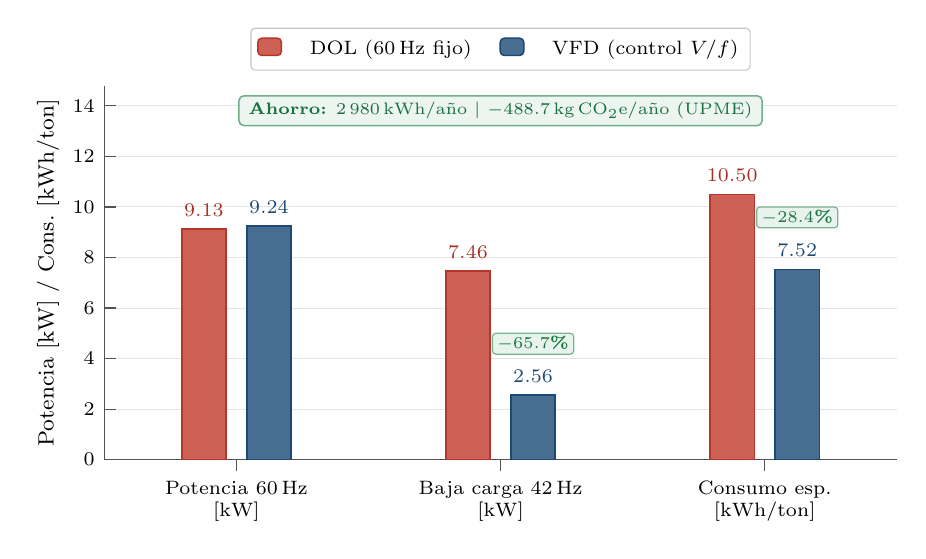
\begin{tikzpicture}
\begin{axis}[
    ybar=7.5pt,
    bar width=16pt,
    scale only axis,
    width=0.83\linewidth,
    height=4.75cm,
    ymin=0, ymax=14.8,
    ytick={0,2,4,6,8,10,12,14},
    symbolic x coords={p60,p42,cesp},
    xtick=data,
    xticklabels={
        {Potencia 60\,Hz\\{[kW]}},
        {Baja carga 42\,Hz\\{[kW]}},
        {Consumo esp.\\{[kWh/ton]}}
    },
    enlarge x limits=0.25,
    ylabel={Potencia [kW] / Cons.\ [kWh/ton]},
    ymajorgrids=true,
    grid style={gray!20, line width=0.35pt},
    axis x line*=bottom,
    axis y line*=left,
    axis line style={gray!65!black, line width=0.55pt},
    tick style={gray!65!black, line width=0.45pt},
    tick label style={font=\scriptsize},
    x tick label style={align=center, yshift=0pt},
    label style={font=\footnotesize},
    ylabel style={yshift=-2pt},
    nodes near coords,
    nodes near coords align={vertical},
    every node near coord/.append style={
        font=\scriptsize\bfseries,
        yshift=1pt,
        /pgf/number format/fixed,
        /pgf/number format/fixed zerofill,
        /pgf/number format/precision=2
    },
    legend style={
        at={(0.5,1.04)},
        anchor=south,
        legend columns=2,
        font=\scriptsize,
        draw=gray!45,
        fill=white,
        inner sep=2.2pt,
        column sep=8pt,
        rounded corners=1.5pt
    },
    legend image code/.code={
        \draw[#1] (0cm,-0.08cm) rectangle (0.30cm,0.14cm);
    }
]
\addplot[
    fill=f4Red!80,
    draw=f4Red!95!black,
    line width=0.55pt,
    every node near coord/.append style={text=f4Red!85!black}
] coordinates {
    (p60,9.13)
    (p42,7.46)
    (cesp,10.50)
};
\addlegendentry{DOL (60\,Hz fijo)}

\addplot[
    fill=f4Blue!82,
    draw=f4Blue!95!black,
    line width=0.55pt,
    every node near coord/.append style={text=f4Blue!95!black}
] coordinates {
    (p60,9.24)
    (p42,2.56)
    (cesp,7.52)
};
\addlegendentry{VFD (control $V/f$)}

% Indicadores porcentuales centrados sobre cada barra VFD (bar shift = +(16+7.5)/2 = +11.75pt)
\node[
    anchor=south,
    xshift=11.75pt,
    font=\fontsize{6.0}{6.8}\selectfont\bfseries,
    text=f4Green!90!black,
    fill=f4Green!10,
    draw=f4Green!60,
    line width=0.45pt,
    rounded corners=1.2pt,
    inner xsep=1.7pt,
    inner ysep=1.1pt
] at (axis cs:p42,4.15) {$-65.7$\symbol{37}};

\node[
    anchor=south,
    xshift=11.75pt,
    font=\fontsize{6.0}{6.8}\selectfont\bfseries,
    text=f4Green!90!black,
    fill=f4Green!10,
    draw=f4Green!60,
    line width=0.45pt,
    rounded corners=1.2pt,
    inner xsep=1.7pt,
    inner ysep=1.1pt
] at (axis cs:cesp,9.15) {$-28.4$\symbol{37}};

% Recuadro informativo anualizado en la zona superior libre (sin recortes laterales)
\node[
    anchor=north,
    font=\fontsize{6.5}{7.5}\selectfont,
    text=f4Green!85!black,
    fill=f4Green!8,
    draw=f4Green!65,
    line width=0.55pt,
    rounded corners=1.8pt,
    inner xsep=3.5pt,
    inner ysep=2.4pt,
    align=center
] at (rel axis cs:0.5,0.975) {\textbf{Ahorro:} 2\,980\,kWh/año \textbar{} $-488.7$\,kg\,CO$_2$e/año (UPME)};
\end{axis}
\end{tikzpicture}
\par\vspace{3pt}
{\footnotesize (b) Potencia activa (60\,Hz vs.\ 42\,Hz) y consumo específico.}
\end{minipage}
\caption{Comparación electromecánica y energética del arranque directo en línea (DOL) frente al variador de frecuencia (VFD, rampa de 6\,Hz/s) simulada en Godot~4.7.2 (\texttt{InductionMotorKloss.gd} y \texttt{VFDDriveController.gd}) para el motor trifásico de 10\,HP: (a) transitorio de corriente eficaz $I_{\mathrm{rms}}(t)$ y velocidad rotórica $N_r(t)$, destacando la reducción del pico de rotor bloqueado $I_{\mathrm{LRA}}=81.4\,\mathrm{A}$ respecto a la nominal $I_{\mathrm{FLA}}=13.5\,\mathrm{A}$; (b) potencia activa a plena carga (60\,Hz, 0.8\,kg/s), ahorro por ley cúbica a baja carga (42\,Hz, $-65.7\%$) y consumo específico ($-28.4\%$), con impacto anual estimado según factor de emisión UPME.}
\label{fig:vfd_vs_dol}
\end{figure*}
